\documentclass[a4paper,11pt]{article}
\usepackage{f420}

\newtheorem{statement}{Утверждение}
\newtheorem{algo}{Алгоритм}
\begin{document}

По статье "The Geometry of Binary Search Trees" от Demaine, Harmon, Iacono, Kane, Pătrașcu (SODA, 2010).

\section{Введение}

Буквы~$n$ и~$m$ всегда обозначают размер BST и общее количество выполненных операций поиска соответственно.

\subsection{BST}

В нашей модели вычислений за одно действие можно взять какое-то поддерево, которое затрагивает корень и произвольно его преобразовать (сохраняя свойство BST).
\begin{definition}[Переконфигурация]
Пусть дано бинарное дерево поиска (BST)~$T_1$, поддерево~$\tau$ дерева~$T_1$, содержащее корень, и дерево~$\tau'$ на тех же узлах, что и~$\tau$. Скажем, что~$T_1$ может быть преобразовано с помощью операции~$\tau \to \tau'$ в другое BST~$T_2$, если~$T_2$ идентично~$T_1$, за исключением замены~$\tau$ на~$\tau'$. Стоимость такой переконфигурации определяется как~$|\tau| = |\tau'|$.
\end{definition}

\begin{definition}[Исполнение BST]
Пусть задана поисковая последовательность $S = \langle s_1, s_2, \dots, s_m \rangle$. Скажем, что алгоритм BST выполняет~$S$ через исполнение~$E = \langle T_0, \tau_1 \to \tau'_1, \dots, \tau_m \to \tau'_m \rangle$, если все переконфигурации допустимы и~$s_i \in \tau_i$ для всех~$i$ (т.е. поиск таки нашел запрашиваемый элемент $s_i$). 

Для~$i = 1, 2, \dots, m$ определим~$T_i$ как~$T_{i-1}$ с переконфигурацией~$\tau_i \to \tau'_i$. Стоимость выполнения~$E$ задается как~$\sum_{i=1}^{m} |\tau_i|$.
\end{definition}


Данная модель эквивалентна другим моделям BST с точностью до постоянного множителя. Например, другой способ моделирования дерева поиска заключается в представлении каждой операции поиска как начинающейся с указателя на корень, с использованием следующих элементарных операций с фиксированной стоимостью: перемещение указателя к левому потомку, перемещение указателя к правому потомку, перемещение указателя вверх, правый поворот в точке указателя, левый поворот в точке указателя. 
Эта эквивалентность сохраняется, поскольку любое BST может быть преобразовано в любое другое BST с теми же узлами за линейное время.

\subsection{Арбореально удовлетворенные множества} 
Переходя к геометрической интерпретации, точка~$p$ обозначает точку на плоскости с целочисленными координатами~$(p.x, p.y)$, удовлетворяющими условиям~$1 \leq p.x \leq n$ и~$1 \leq p.y \leq m$. Обозначим за~$\square ab$ оси-ориентированного прямоугольника с вершинами~$a$ и~$b$ (включая границы и внутренность).

\begin{definition}
Пара точек~$(a, b)$ (или индуцированный ими прямоугольник~$\square ab$) является \emph{арбореально\footnote{Термин происходит от латинского слова arbor, что означает «дерево». Он используется в различных контекстах для описания чего-то, связанного с деревьями или имеющего древовидную структуру.} удовлетворенной} относительно множества точек~$P$, если выполняется одно из следующих условий: 
(1) точки~$a$ и~$b$ ортогонально коллинеарны (горизонтально или вертикально выровнены); 
(2) в~$\square ab$ содержится хотя бы одна точка из~$P \setminus \{a, b\}$. 
\end{definition}
\begin{definition}
Множество точек~$P$ называется \emph{арбореально удовлетворенным}, если каждая пара точек в~$P$ является арбореально удовлетворенной относительно~$P$.
\end{definition}

\begin{statement} \label{obs:arb_satisfaction}
\textit{В арбореально удовлетворенном множестве точек~$P$ для любых~$a, b \in P$, которые не являются ортогонально коллинеарными, существует хотя бы одна точка из~$P \setminus \{a, b\}$ на сторонах~$\square ab$, инцидентных~$a$, и хотя бы одна точка на сторонах, инцидентных~$b$. (Эти две точки могут совпадать.)}
\end{statement}

\begin{proof}
Рассмотрим любые две точки~$a, b \in P$, которые не являются ортогонально коллинеарными. Так как~$\square ab$ является удовлетворенным, он содержит некоторую точку~$c \in P$. Если~$c$ не находится на стороне~$\square ab$, инцидентной~$a$, тогда мы можем рекурсивно перейти к~$\square ac$, пока не найдем такую точку. Аналогично, если~$c$ не находится на стороне~$\square ab$, инцидентной~$b$, то мы можем рекурсивно перейти к~$\square cb$, пока не найдем такую точку.
\end{proof}

Теперь мы визуализируем выполнение алгоритма BST интуитивным способом: на момент времени~$i$ (в строке~$i$) мы отображаем все узлы, затронутые в~$\tau_i$. Модель BST была выбрана так, чтобы игнорировать лишь несущественные детали (например, точные повороты и перемещения указателя), что упрощает геометрическую интерпретацию.

\begin{definition}
	\emph{Геометрическое представление выполнения} BST~$E$ задается как множество точек~$P(E) = \{(x, y) \mid x \in \tau_y\}$.
\end{definition}

\begin{lemma} \label{lemma:bst_arborall}
Множество точек~$P(E)$ для любого выполнения BST является арбореально удовлетворенным.
\end{lemma}

\begin{proof}
	Предположим противное, а именно, что существуют~$a \in \tau_i$ и~$b \in \tau_j$ при~$i < j$ и~$a \neq b$, и при этом никакие другие узлы в отрезке~$[a, b]$ не были затронуты во временном интервале~$[i, j]$. Обозначим через~$c$ наименьшего общего предка~$a$ и~$b$ в дереве~$T_i$. Рассмотрим два случая:

\begin{itemize}
	\item Если~$c \neq a$, то~$c$ должно быть затронуто в момент времени~$i$, чтобы добраться до~$a$ ($c \in \tau_i$), и~$c \in (a, b]$ . Получаем противоречие.
    
	\item Если~$c = a$, то в момент времени~$i$ узел~$a$ является предком~$b$. По предположению, что~$\square ab$ не удовлетворено, узел~$b$ не затрагивается в промежутке времени $[i, j)$. Следовательно,~$a$ остается на пути к~$b$, то есть~$a$ должен быть предком~$b$ в~$T_j$ и будет затронут, что противоречит условию~($a \in \tau_j$).
\end{itemize}
\end{proof}

\section{Оффлайн-эквивалентность}

Геометрическая интерпретация представляется как весьма упрощённое представление выполнения BST, так как она отражает только множество узлов в~$\tau_i$ и не указывает, каким образом эти узлы должны быть перестроены с помощью поворотов.  
Довольно неожиданно оказывается, что точная форма дерева не является существенной информацией и может быть восстановлена лишь на основе множеств затронутых узлов! Другими словами, можно реконструировать последовательность выполнения по любому геометрическому представлению, удовлетворяющему необходимому условию арбореальной удовлетворённости.

\begin{lemma} \label{lemma:arboral_bst}
	Для любого арбореально удовлетворенного множества точек~$X$ существует выполнение BST~$E$ такое, что~$P(E) = X$. Назовём~$E$ арбореальным представлением~$X$ и обозначим~$P^{-1}(X) = E$.
\end{lemma}

\begin{proof}
	Опишем алгоритм для обратного преобразования~$P^{-1}(\cdot)$, смотреть Картинку \ref{fig:geometry}. 
Определим \emph{время следующего доступа}~$N(x, i)$ для~$x$ в момент времени~$i$ как минимальную координату~$y$ среди всех точек в~$X$ на луче от~$(x, i)$ до~$(x, \infty)$. Если такой точки нет, положим~$N(x, i) = \infty$.

Пусть~$T_i$ — это Декартово дерево, построенное на всех точках~$(x, N(x, i))$. Напомним, что Декартово дерево представляет собой BST по первой координате и кучу по второй, где совпадающие значения разрешаются произвольно. Таким образом,~$T_i$ является корректным BST на~$n$ значениях, удовлетворяющим свойству кучи согласно времени следующего доступа (с минимумом в корне).

Пусть~$\tau_i$ — это точки в~$X$ с~$y = i$. По свойству Декартового дерева~$T_i$, множество~$\tau_i$ должно образовывать связное поддерево~$T_i$, включающее корень (так как~$i$ является минимальным возможным временем доступа~$N(\ast, i)$). Далее, формируем~$T_{i+1}$, переставляя узлы в~$\tau_i$ так, чтобы они образовали Декартово дерево, основанное на времени следующего доступа~$(x, N(x, i+1))$. 

Покажем, что~$T_{i+1}$ является Декартовым деревом на~$(x, N(x, i+1))$. Свойство BST выполняется по построению, поэтому рассмотрим свойство кучи. Достаточно показать, что оно выполняется для каждой пары родитель/потомок~$(q, r)$ в~$T_{i + 1}$. 
Если оба узла находятся в~$\tau_i$, то свойство кучи сохраняется по построению. Если оба узла находятся вне~$\tau_i$, то их время следующего доступа и их отношение родитель/потомок не изменились при переходе от~$i$ к~$i+1$, а значит, свойство кучи также выполняется. Остаётся случай, когда~$q \in \tau_i$, а~$r \notin \tau_i$. Однако если свойство кучи нарушается в~$T_{i+1}$, то прямоугольник от~$(q, i)$ до~$(r, N(r, i))$ противоречит Утверждению~\ref{obs:arb_satisfaction}: вертикальная сторона при~$x = q$ пуста, поскольку~$N(q, i+1) > N(r, i)$ (в силу предположения о нарушении свойства кучи). 
Горизонтальная сторона при~$y = i$ также пуста, так как в противном случае найдется некий $x \neq  q$ на этой стороне и тогда $r, q$ были бы в разных ветвях относительно $x$ в дереве $T_{i + 1}$,  противоречие.
\end{proof}

Пусть \emph{геометрическое представление} последовательности доступа~$S$ определяется как множество точек~$P(S) = \{(s_1,1), (s_2,2), \dots, (s_m,m)\}$. 
Леммы~\ref{lemma:bst_arborall} и~\ref{lemma:arboral_bst} показывают, что арбореальное утверждение <<$E$ выполняет~$S$>> эквивалентно геометрическому утверждению <<$P(S) \subseteq P(E)$>>. 
Обозначим через~$\operatorname{minASS}(S)$ размер наименьшего арбореально удовлетворённого над-набора множества~$P(S)$. Тогда имеем $\operatorname{OPT}(S) = \operatorname{minASS}(P(S))$. Таким образом, вопрос того чтобы находить/аппроксимировать $\mathrm{OPT}(S)$ эквивалентен разработке алгоритмов для поиска минимального арбореально удовлетворённого над-набора.

\section{Онлайн-эквивалентность} 

Выше мы установили комбинаторную эквивалентность между деревьями поиска и арбореально удовлетворёнными множествами, тем самым охарактеризовав офлайн-алгоритмы BST. 
Теперь мы стремимся усилить эту характеристику для \emph{онлайн}-алгоритмов BST, которые должны выполнять преобразование~$\tau_i \to \tau'_i$ после каждого $s_i$ без доступа к последующим запросам.

\begin{definition}
Задача \emph{онлайн-арбореально удовлетворённого над-набора} (online ASS) заключается в разработке алгоритма, который получает множество точек~$\{(s_1,1), (s_2,2), \dots, (s_m,m)\}$ поступательно. 

После получения точки~$i$ алгоритм должен вывести множество~$P_i$ точек на линии~$y = i$ так, чтобы 
\[
\{(s_1,1), (s_2,2), \dots, (s_i,i)\} \subseteq P_1 \cup P_2 \cup \dots \cup P_i
\]
было арбореально удовлетворённым. Стоимость алгоритма определяется как~$\sum_{i=1}^{n} |P_i|$.
\end{definition}


Онлайн-алгоритм BST естественным образом определяет онлайн-алгоритм ASS через стандартное геометрическое представление (Лемма~\ref{lemma:bst_arborall}). Обратное утверждение не столь очевидно, так как Лемма~\ref{lemma:arboral_bst} требует знания будущих доступов: она реконструирует форму дерева, накладывая порядок кучи, основанный на будущих временах доступа. Однако, используя следующую концепцию, мы сможем <<угадывать>> форму дерева динамически, теряя лишь постоянный множитель во времени работы.

\begin{definition}
	\emph{Split-дерево} — это абстрактный тип данных, реализующий две операции в модели BST:
\begin{itemize}
    \item \texttt{MakeTree}$(x_1, x_2, \dots, x_n)$~--- создаёт BST из~$n$ узлов на основе заданных значений.
    \item \texttt{Split}$(x)$~--- перемещает~$x$ в корень дерева, а затем удаляет его, оставляя левые и правые поддеревья корректными split-деревьями.
\end{itemize}
\end{definition}

\begin{statement}
	Split-деревья можно реализовать с худшим случаем стоимости~$O(n)$ для \texttt{MakeTree} и произвольной последовательности из~$n$ операций \texttt{Split} (т.е. амортизировано $O(1)$).
\end{statement}
\begin{proof}
	Опущен.
\end{proof}

\begin{lemma} \label{lemma:online_bst_arborall}
Для любого онлайн-алгоритма ASS~$A$ существует онлайн-алгоритм BST~$A'$, такой что для любой последовательности доступа стоимость~$A'$ ограничена сверху константным множителем от стоимости~$A$.
\end{lemma}
\begin{proof}
Основная идея заключается в том, что когда нам нужно сохранить множество элементов в некотором неизвестном будущем порядке, мы избегаем принятия решений и храним их в split-дереве. Получаемая конструкция может рассматриваться как инверсия доказательства Леммы~\ref{lemma:bst_arborall}, поскольку split-деревья хранятся в порядке кучи по времени предыдущего доступа (вместо времени следующего доступа).

Формально, пусть~$\rho(x, i)$ — это время последнего доступа к~$x$ перед~$i$, то есть~$y$-координата наивысшей точки на луче от~$(x, i)$ до~$(x, -\infty)$. Если такой точки нет, полагаем~$\rho(x, i) = -\infty$. 
Обозначим через~$G_i$ \emph{общее Декартово дерево}, определённое на всех точках~$(x, \rho(x, i))$, то есть BST по координатам~$x$ и \emph{общий heap} по~$\rho(x, i)$ (в этот раз на максимум). В общем heap'е совпадающие ключи объединяются в \textit{суперузел} с несколькими значениями.
Т.е. каждая вершина Декартового дерева это множество элементов с одинаковым $\rho(x, i)$ ключи которых хранятся в split-дереве.

Рассмотрим, как эта структура изменяется при переходе от момента времени~$i$ к~$i+1$. Все точки на строке~$y = i+1$ будут иметь~$\rho(x, i+1) = i+1$ и будут перемещены из~$G_i$ в корень~$G_{i+1}$. 

Ключевое свойство, вытекающее из арбореальной удовлетворённости (и которым мы уже пользовались в Лемме~\ref{lemma:bst_arborall}) это то, что вершины с $\rho(x, i + 1) = i + 1$ будут образовывать связный подграф включающий корень в $G_{i + 1}$. 
Действительно, пусть есть такая тройка вершин $a < b < c$, что $\rho(a, i + 1) = \rho(c, i + 1) = i + 1$ и $\rho(b, i + 1) < i + 1$ и при этом $b$ лежит между $a, c$.
Значит, $c$ находится внутри 

Это означает, что мы можем переместить все соответствующие значения в корень одним обходом дерева от корня к листьям. На каждом суперузле мы вызываем \texttt{Split} для выделения запрашиваемых узлов, формируя новый скелетный узел и два дочерних суперузла. Затем все собранные скелетные узлы объединяются в корневой суперузел с помощью \texttt{MakeTree}. 

Поскольку каждая операция \texttt{Split} имеет амортизированную константную стоимость, а \texttt{MakeTree} выполняется за линейное время, общая стоимость моделирования доступа на строке~$y = i$ пропорциональна числу точек на этой строке.
\end{proof}

\section{Greedy Future}

Данный кусок не был затронут на лекции.

\begin{algo} [\textsc{GreedyFuture} (\textsc{GF}) Algorithm] \label{algorithm:greedy_future}
    \textbf{Input:} Последовательность запросов~$X \in [n]^m$ и начальное BST~$T_0$. 
    Мы перестраиваем~$T_{t-1}$ в~$T_t$ после обработки запроса~$x_t$ с~$T_{t-1}$ для~$t = 1, \dots, m$.

    \textbf{Function} \textsc{Restructure}(\textit{запрос }~$v$, \textit{дерево }~$T_{t-1}$, \textit{будущие запросы }~$X'$):

    \begin{algorithmic}[1]
        \State Пусть $v_1 < v_2 < \dots < v_k$ — узлы на пути от корня~$T_{t-1}$ до запрашиваемого значения~$v$ (включая~$v$ и корень). 
        \State Определим $v_0 = -\infty$ и $v_{k+1} = +\infty$.
        \State Обозначим поддеревья, отходящие от этого пути, как $R_0, \dots, R_k$.
		\State Положим $\tau(v_i)$ — индекс первого появления запроса значения $x \in (v_{i-1}, v_{i+1})$ в~$X'$ для каждого $i \in [k]$.

        \State Переструктурируем узлы $v_1, \dots, v_k$ в Декартово дерево:
        \begin{itemize}
            \item Дерево поддерживает порядок BST.
            \item Приоритеты в heap'е определяются значениями $\tau$, где корень имеет наименьшее $\tau$.
            \item При равных значениях предпочтение отдаётся, например, меньшим ключам или узлам с меньшей глубиной до реструктуризации.
        \end{itemize}
        
        \State Подвесим поддеревья $R_0, \dots, R_k$ на их соответствующие позиции.
        
        \State Возвращаем полученное дерево $T_t$.
    \end{algorithmic}
\end{algo}

Данный жадный алгоритм предполагался как такой, что работает лучше любого онлайн алгоритма.
Оказывается, что его можно сделать онлайн с потерей в константный множитель.

\begin{algo} \label{algorithm:greedy_ass}
Проводим сканирующую горизонтальную линию по множеству точек в порядке увеличения координаты~$y$. В момент времени~$i$, \textsc{GreedyASS} добавляет минимальное количество точек на~$y = i$, чтобы множество точек вплоть до~$y \leq i$ стало арбореально удовлетворённым.

\textit{Этот минимальный набор точек определяется однозначно: для любого неудовлетворённого прямоугольника, содержащего~$(s_i, i)$ в одном из углов, добавляется противоположный угол при~$y = i$.}
\end{algo}

\begin{theorem}
	При применении Леммы~\ref{lemma:arboral_bst} к Алгоритму~\ref{algorithm:greedy_ass} получается Алгоритм~\ref{algorithm:greedy_future}.
\end{theorem}
\begin{proof}
	Доказательство по индукции, на очередном шаге $(s_i, i)$ достаточно показать, что Алгоритм~\ref{algorithm:greedy_ass} достроит ровно те точки, которые в дереве Алгоритма~\ref{algorithm:greedy_future} будут на пути от корня до $s_i$. 
	Далее, по Лемме~\ref{lemma:arboral_bst} на этом пути построится Декартово дерево, также как и в обычном GF.

	Рассмотрим вершину $v$ на пути от корня до $s_i$ в дереве $T_{i - 1}$ и пусть $j$ ~-- момент когда последний раз к ней был доступ.
	Пусть $\square (s_i, i) (v, j)$ арбореально удовлетворённый, тогда найдется некая точка $(c, k)$ на границе этого прямоугольника.
	Тогда $k = j$, ведь иначе бы мы взяли точку $v$ повыше.
	Но тогда $c$ лежит строго между $s_i, v$. 
	А следовательно, путь прошел бы по нему.
	В обратную сторону, аналогично.
\end{proof}

Заметим, что Алгоритм~\ref{algorithm:greedy_ass} не смотрит в будущее.
Этот~онлинифицированный вариант «максимально оффлайнного» алгоритма, по-видимому, указывает на~то, что~оффлайн-алгоритмы не~могут асимптотически превосходить лучшие онлайн-алгоритмы в~модели BST, то~есть динамическая оптимальность возможна.

\newpage
\begin{figure}[htpb]
	\centering
	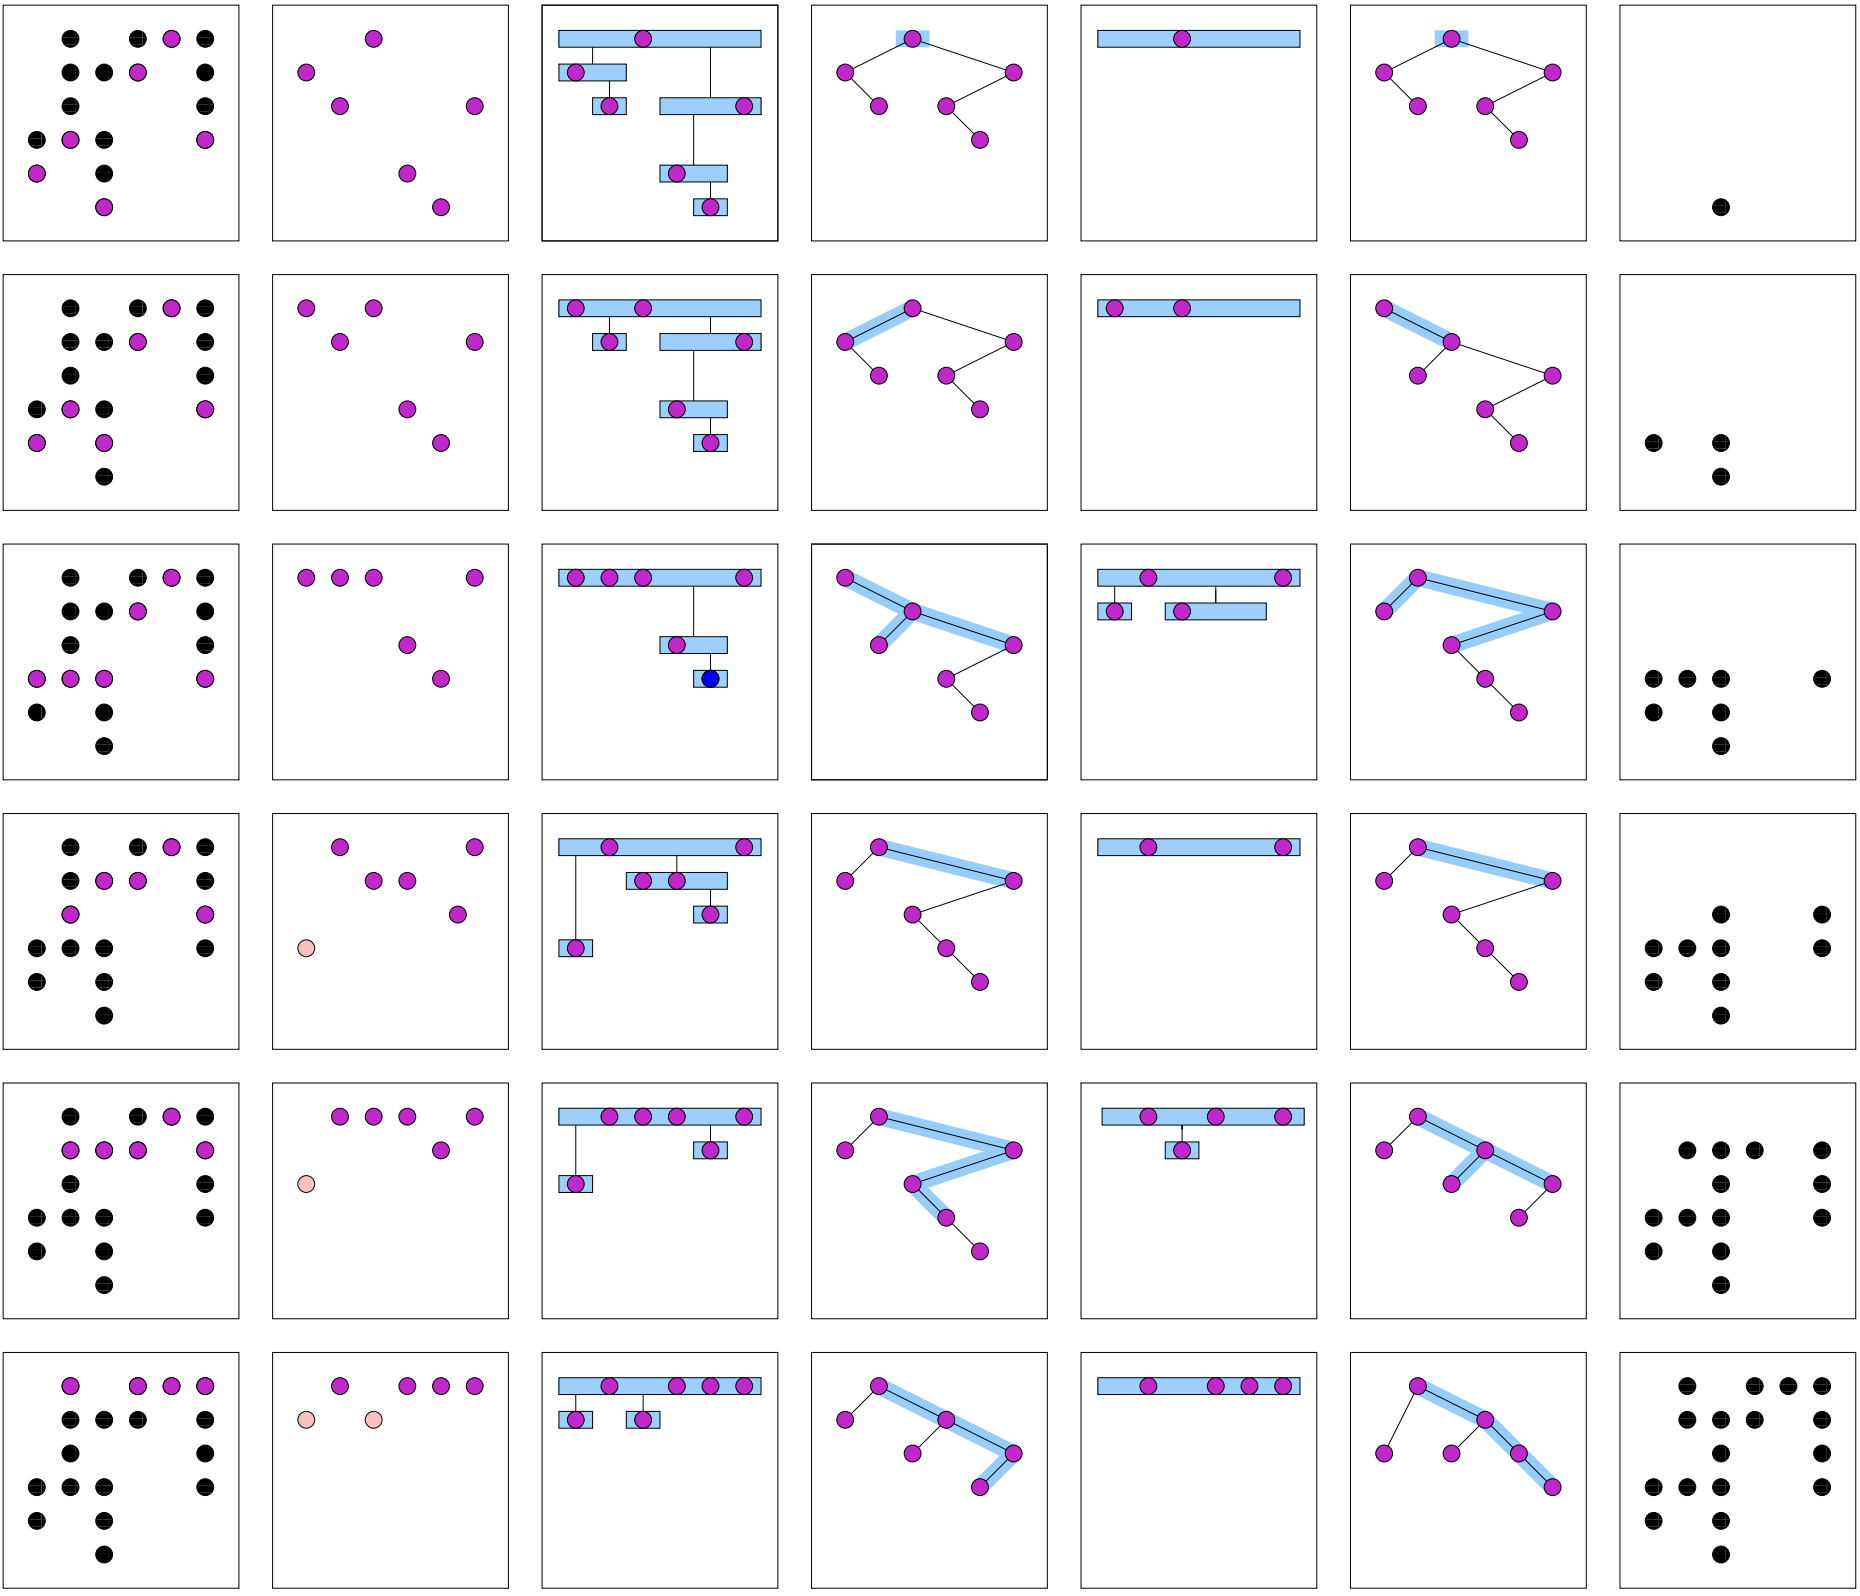
\includegraphics[width=0.8\textwidth]{img/geometry.png}
	\caption{Иллюстрация преобразований между деревом и геометрическим представлением. Колонки слева направо:
(1) Множество точек~$X$; в строке~$i$ светлые узлы представляют появления, определяющие~$N(x, i)$. 
(2) Светлые узлы из колонки~1 перерисованы и отражены по вертикали для упрощённого преобразования в дерево; ещё более светлые узлы, для которых~$N(x, i) = \infty$, располагаются внизу.
(3) Общее Декартово дерево. 
(4) Дерево~$T_{i-1}$. 
(5) Декартово Дерево, сформированное по времени следующего доступа узлов~$\tau_i$ в момент~$i+1$ (произвольная бинаризацию).
(6) Дерево~$T_i$.
(7) затенённые узлы~$\tau$ из колонок~4 или~6, восстанавливая исходное множество точек из колонки~1.}
	\label{fig:geometry}
\end{figure}


\end{document}
